\section{High-Level Architektur}
\label{sec:HighLevelArchitektur}  

%A multi-tenant management system must fulfill several requirements, such as data and performance isolation between tenants and users, authentication, specification of different user roles, resources usage monitoring, etc. In a \ac{JBI} environment, endpoint and routing configurations files are packed in \ac{SU}s, and the latter in \ac{SA}s for deployment. However, there is a lack of user-specific data during deployment. Muhler solves this problem in JBIMulti2 by injecting tenant context in the \ac{SA} packages, making them tenant-aware \cite{Muhler2012}. 

%\begin{figure}[htb]
%	\centering
%		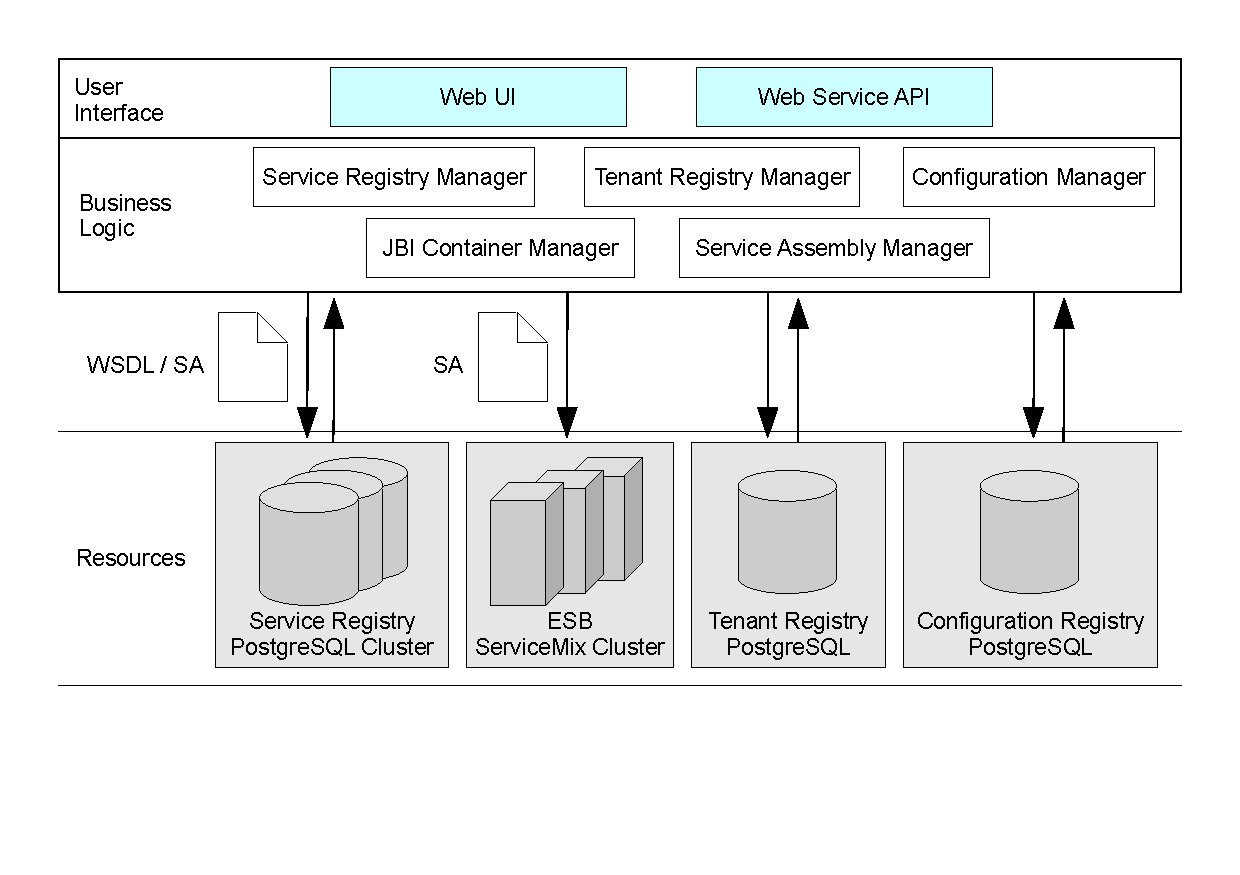
\includegraphics[clip, scale=0.5]{./gfx/systemoverview_jbimulti2.pdf}
%	\caption[JBIMulti2 System Overview]{JBIMulti2 System Overview \cite{Muhler2012}} 
%	\label{fig:jbimulti2}
%\end{figure}

%The architecture of the JBIMulti2 system is represented in Figure \ref{fig:jbimulti2}. We can distinguish two main parts in the system: business logic and resources. JBIMulti2 uses three registries for storing configuration and management data. When a tenant (or a tenant user) is registered, an unique identification number is given to them and stored in the Tenant Registry. Both Tenant Registry and Service Registry are designed for storing data of more than one deployed application. The former for storing tenant information and the latter for providing a dynamic service discovery functionality between the different applications accessed through the \ac{ESB}. The Configuration Registry is the key of the tenant isolation requirement of the system. Each of the stored tables are indexed by the tenant id  and user id value. In this thesis we need tenant information during runtime. We reuse and extend the databases schemas produced by Muhler, specifically the Service Registry.

%The system provides a user interface for accessing the application's business logic. Through the business logic, the management of tenants can be done by the system administrator or the management of tenant's users can be done by the tenants. Furthermore, when deploying the different tenant's endpoint configurations packed in \ac{SA}s, the system first makes modifications in the zip file for adding tenant context information and then communicates with the Apache ServiceMix instance by using a \ac{JMS} Topic to which all the ServiceMix instances are subscribed to. The \ac{JMS} management service in ServiceMix deploys the received \ac{SA} injected in the received \ac{JMS} message using the administration functionalities provided in ServiceMix. The communication between the business layer and the ServiceMix instance is unidirectional. When successful deployment, the endpoint is reachable by the tenant. When an error occur during deployment, an unprocessed management message is posted in a dead letter queue.

%JBIMulti2 requires the previous installation of components, e.g. JOnAS server, PostgreSQL, etc. The initialization of the application is described in both Chapter \ref{chap:validationevaluation} and in the JBIMulti2 setup document \cite{JBIMulti2Man}.

BigData4Biz wird hergestellt um gerade und zukünftig bei namhaften Kunden eingesetzt zu werden. Um diese Software langlebig und nachhaltig zu betreiben, ist die Herstellung einer Architektur nötig. \cite{SHR11} behauptet, dass die Architektur eines Systems die Strukturen des Systems, dessen Bausteine, Schnittstellen und deren Zusammenspiel beschreibt.  Dies Bedeutet, dass eine Architektur die Systembausteine sowie ihre Beziehungen zueinander zum einen vorstellt und zum anderen zeigt die Gruppierung von diesen Bausteinen sowie die Bausteine gehörenden Schnittstellen. Eine Architektur hilft dabei nicht nur einen Überblick über die Struktur eines Systems zu haben durch die grobe Anzeige von nur wichtige Aspekte des Systems, sondern auch zur wartbare, flexible, verständliche und langfristige Konstruktion von diesem.

In Abbildung \ref{fig:ArchitekturBD4B} wird die Architektur von BigData4Biz gezeigt. Hier wird keine konkrete Plattformkommunikationstechnologie vorgestellt, sondern die generellen Elemente, die wichtig sind für die Funktionsweise.

%\begin{figure}
%	\centering
%	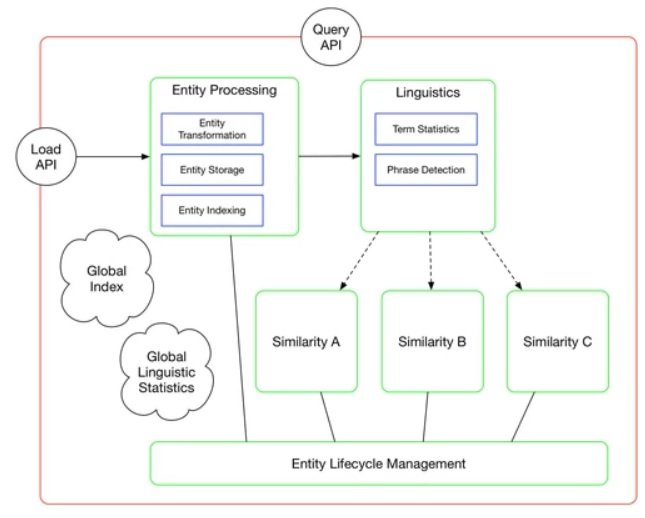
\includegraphics[clip, scale=0.6]{./gfx/Architecture_BD4B.jpg}
%	\caption[High-Level-Architektur von BigData4Biz ]{High-Level-Architektur von BigData4Biz \cite{DIB18} 
%	\label{fig:ArchitekturBD4B}
%\end{figure}


\begin{enumerate}
	\item Die Datenquelle (1) ist ein wichtiger Teil der Architektur, der sich aber nicht in BigData4Biz befindet, sondern bei der Kundenseite. Diese entspricht eine physische Instanz, an der Daten generiert werden. Eine relationale Datenbank, ein Dateisystem, eine Ereignisquelle oder eine Webseite sind Beispiele von Datenquellen. Das Ziel der Datenquelle ist die Sammlung aller technischen Informationen, die einen Zugriff auf Informationen ermöglichen. Die Existenz von mehreren Datenquellen für eine physische Quelle zur Unterscheidung der logischen Partitionierung von Daten an der physischen Quelle, ist möglich. Die Datenquelle ist mit einer standardisierten Übertragungsschnittstelle versehen und enthält unterschiedliche Entitäten (2) und Agenten (5), die wichtig sind für die spätere Ausnutzung von Daten in BigData4Biz. Für die Datenquelle die Ausgabe von Entitäten verschiedener Klassifizierungen und Strukturen ist möglich.
	\item Die Entität (2) stellt die primär verknüpften Daten in BigData4Biz und ist ähnlich zu einer Ressource in der Terminologie von verknüpften offenen Daten und Resource Description Framework (RDF) [DIB18]. Es besteht jedoch eine starke Unterscheidung zwischen die Datenquellen der Entitäten, ihre Verwendung und die verknüpften offenen Daten. Die Datenquelle liefert die Darstellung eines beliebigen Datenelementes aus einer Datenquelle und entspricht ein relationaler Datensatz, ein Join von Beziehungsdatensätzen, eine Datei, eine Webseite, ein Text oder allgemein strukturierte Daten aller Art. BigData4Biz kann die Berechnung der Beziehung zwischen eine Subjektentität und eine Objektentität durchführen. Es sei denn eine Verknüpfung der Subjektentität über ein Prädikat mit einer Objektentität erfolgt und die Begründung von verschiedenen Arten von Ähnlichkeiten zwischen Subjekt und Objekt ist durch das Prädikat möglich. Daten werden in einer Entität (2) durch Agenten (3) umgewandelt um später in BigData4Biz über eine Lade-API (5) geladen zu werden zur Durchführung der Dokumentähnlichkeitsbestimmung. Sobald eine Entität in BigData4Biz empfangen und gespeichert wird, besitzt diese Informationen wie die Entitätsbezeichnung, die Datenquellenbezeichnung, der Agentenname, das Backlink, Metadaten und Eigenschaften.
	\item Die Übertragung der Entitäten (2) von einer Datenquelle (1) zu BigData4Biz erfolgt in der Extract-Transform-Load (ETL)- Methode. Jedoch gibt es keine festgelegte Implementierung von diesem ETL-Schritt, wo es ausnahmsweise die Lade-API (5) gibt, deren erwarteten Aufgabe den Empfang von Entitäten (2) ist. Die Entitätsagenten (3) werden benutzt von der gebräuchlichsten Implementierung des ETL. Die Entitätsagenten entsprechen kleine Programme mit Zugriff auf eine Datenquelle, erhöhten Rechte, und die die Ermittlung von neuen oder geänderten Daten durchführen. Der Entitätsagent (3) führt die Umwandlung der extrahierten Daten in die Entitätsform selbst durch. Der Entitätsagent (3) befindet sich in der Sicherheitszone der Datenquelle (1) zur effektiven Erkennung der Datenänderungen und einfachere Sendung von Daten. Es bestehen schon definierte Standardagenten für allgemeine physische Datenquelle (1), die den vollständigen ETL-Schritt liefern. Die Entitätsagenten (3) sind Buchhalter aller aus ihrer Datenquelle (1) extrahierte Entitäten. Damit können Datenänderungen an Entitäten in BigData4Biz verfolgt werden und die Entität kann zum Zeitpunkt des Ladens aktualisiert werden.
	
	\item Abfrage-API (4) dafür da eine Interaktion zwischen BigData4Biz und den Nutzer zu ermöglichen und entspricht einen REST-fähiger Dienst, der dazu dient verbundene Einblicke in die geladenen Entitäten abzufragen. Es können hier traditionelle Suche nach Entitäten mit Phrasen oder Textausschnitten durchgeführt werden im Rahmen von Abfragen. Die Umwandlung eines gefundenen Interessenbereichs in einen neuen Bereich, wo Ähnlichkeitsbeziehungen, zusätzliche Ausdrücke oder eine Auswahl signifikanter Ausdrücke des Geltungsbereichs benutzt werden, ist möglich. In einem Bereich befinden sich einige Sehenswürdigkeit darstellende dedizierte Entitäten und einen Kontext von zum Definieren von Ähnlichkeitsbeschränkungen verwendete Entitäten.
	
	\item Die Lade-API (5) entspricht ein REST-konformer Dienst von BigData4Biz, die für den Empfang und die Ladung von Entitäten (2) zur weiteren Verarbeitung in BigData4Biz dient.
	
	\item Die Entitätsverarbeitung (6) ist der Teil der Architektur, der sich um die Entitätsversorgung kümmert in BigData4Biz nachdem diese über die Lade-API (5) geladen wurde. Die Entität wird verarbeitet um passend zu werden für die verschiedenen Algorithmen, die anwesend in BigData4Biz sind. Bei der Entitätsverarbeitung erfolgen die Entitätstransformation (5.a), die Entitätsspeicherung (5.b) und die Entitätsindizierung (5.c). Die Entitätsindizierung (5.c) zum Beispiel ist ein wichtiger Prozess, der die Assoziation eines Vokabulars aus Schlüsselwörtern und allen Dokumenten eines Textkorpus durchführt.
	
	\item Die Linguistik (7) benutzt statistische Informationen über die Texte der Entitäten erstens zur Unterscheidung der signifikante von nicht signifikanten Teilen des Textes und zweitens sowohl zur Bestimmung der Beziehungen von Text auf der lexikalischen Ebene als auch zur Strukturierung von Texten in Gruppen ähnlicher Themen. Dieses Service stellt eine gute grobe Klassifizierung bereit. Dabei wird das Service als Basis statistische Zahlen bezüglich der Häufigkeit und des Auftritts von Begriffen in Dokumente haben und nicht das Verständnis der Bedeutung von Texten. Die Linguistik befindet sich in der Abfrage-API (4), wo ein konkreter Benutzer Suchbegriffe eingeben kann, die später zum Informationenvergleich ausgenutzt werden. Die Verwendung von einer begrenzten Teilmenge der semantischen Analyse wie Teil der Sprachmarkierung für verbesserte Ergebnisse durch signifikante Phrasenextraktion und Begriff gemeinsames Auftreten ist möglich. 
	
	\item Die Ähnlichkeitsdienste (8) berechnen die Ähnlichkeiten zwischen den Dokumenten. Es besteht bei Entitäten eine Subjekt-Prädikat-Objekt-Beziehung (SPO-Beziehung). Die Bestimmung des Prädikates erfolgt nicht durch manuelle Zuweisung oder Berechnung unter Verwendung einer Ontologie. Ähnlichkeitsdienste (8) verfügen über Ähnlichkeitsalgorithmen, die die Berechnung von durch Prädikaten ausgedruckte Ähnlichkeiten durchführen. Die Kernähnlichkeitsalgorithmen von BigData4Biz haben als Basis linguistischen Statistiken (7.a) wie TF-IDF. Die Ähnlichkeitsdienste (8) sind unabhängig von den anderen Diensten und benutzen ihre eigene Persistenz zur effektiven Berechnung von SPO-Beziehungen \cite{DIB18}. 
	
	\item Das Entitätslebenszyklusdienst (9) ist für die Überwachung von jeden schritten der Entitätsverarbeitung (6) zuständig. (Kompletter Teil noch zu ändert: die Nummerzuweisungen wurden geändert [Siehe Abbildung Word Datei])
	
\end{enumerate}



